\chapter{Cassandra}
\label{chap:cassandra}
Cassandra ist die Quelle aller Daten von Twitter, die wir brauchen. Dazu werden die Daten direkt von der Twitter API über Kafka in Cassandra geladen und auf ein vorher für unsere Bedürfnisse zugeschnittenes Datenschema gemappt.

\section{Datenverwaltung}
Wir habe uns entschieden das Twitter Datenschema zu übernehmen. Da allerdings die Twitter Dokumentation nicht genau genug ist und nicht alle Attribute aller Datentypen übersichtlich darstellt, haben wir eine Applikation geschrieben, die sich Tweets vom Twitter Stream holt und daraus das Datenschema im JSON Format zusammenbaut. Nach dem wir die Applikation lange genug laufen lassen haben, hat sich an dem Datenschema nichts mehr geändert und wir konnten die Datentypen extrahieren.\\

\subsection{Datenschema}
\label{subsec:schema}
Nach einer eingehenden Untersuchung aller möglichen Use Cases sind wir zum Schluss gekommen, dass uns fünf Tabellen alle Funktionen bieten, die wir brauchen. Wir haben dabei zwei Tabellen für die User user\_by\_id und user\_by\_screen\_name entworfen wie man in Abbildung \ref{fig:schema} sehen kann.
\begin{figure}[htbp!]
	\centering
	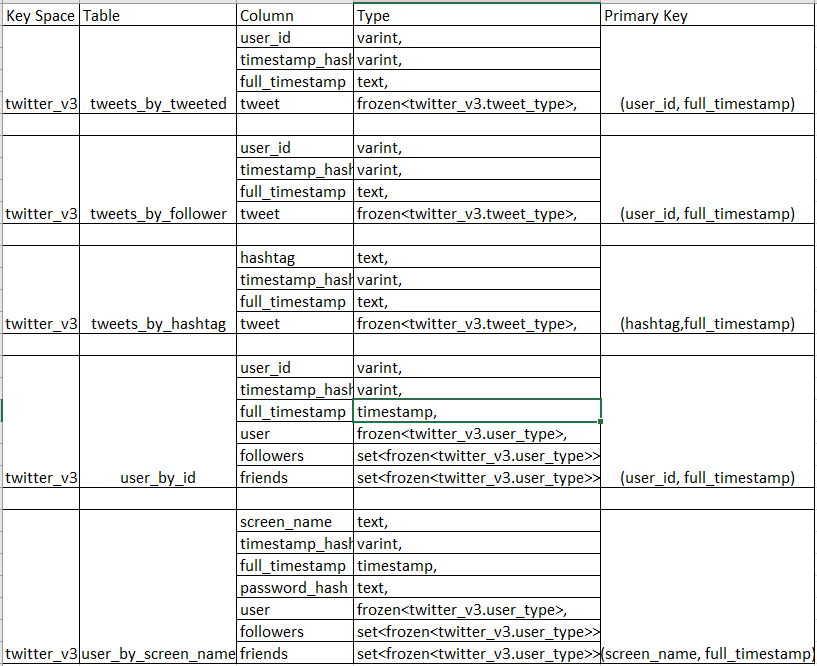
\includegraphics[scale=0.725]{pics/schema.PNG}
	\caption{Cassandra Schema}
	\label{fig:schema}
\end{figure}
Da man bei Cassandra nur über den Primary Key (PK) auf Zeilen zugreifen und Bereichsabfragen über CQL machen kann, gilt es hier den PK so zu wählen, dass alle unsere Funktionen abgedeckt sind. Deshalb haben wir neben der User-Id für user\_by\_id und dem Screen-Name des Users für user\_by\_screen\_name auch den Timestamp mit aufgenommen. Da Cassandra leider keine vollständige Konsistenz bietet, müssen wir uns selber darum kümmern. Durch den Timestamp können wir verschiedene Versionen eines Objektes auseinanderhalten und die neuste bestimmen. Somit können wir zumindest einen gewissen Grad an Konsistenz bieten. Die weiteren Attribute der beiden Tabellen lassen sich einfach erklären. Die Follower und Friends eines Users sind wichtig, um die Timeline zu erstellen. Den password\_hash in user\_by\_screen\_name brauchen wir für den Login.\\
Die anderen drei Tabellen sind dafür da, die Tweets zu speichern und alle Tweet betreffenden Anfragen zu beantworten. Auch hier haben wir wieder den Timestamp bei allen Tabellen mit in den PK aufgenommen um Teilkonsistenz zu gewährleisten. tweets\_by\_tweeted speichert alle Tweets nach der User-Id des Users ab, der den Tweet abgesetzt hat. tweets\_by\_follower hingegen speichert einmal alle Tweets nach User-Id eines jeden Followers ab. Das Konzept hier ist es, durch die mehrfache Speicherung eines Tweets die Zeit bei der Abfrage nach allen Tweets, die ein User auf seiner Timeline sehen kann, zu verkürzen. Da man einmal abgesetzte Tweets auch nicht mehr ändern kann haben wir auch kein Problem damit jedes Objekt für Änderungen wieder heraussuchen zu müssen. tweets\_by\_hashtag speichert dann die Tweets danach ab, welche Hashtags in ihnen verwendet werden. Somit können auch Abfragen über Tweets eines Hashtags effizient beantwortet werden.

\section{Cassandrareader}
Die zentrale Applikation, in der alle Funktionen und Schnittstellen umgesetzt werden ist der Cassandrareader und es ist eine modular aufgebaute in Java geschriebene Anwendung. Als Framework zur Unterstützung von verschiedenen Funktionen haben wir uns für SpringBoot entschieden. SpringBoot hat den Vorteil, dass es eine native API für Kafka besitzt, die es uns so sehr leicht ermöglicht Publisher und Subscriber für Kafka-Topics zu schreiben. So ist die Verbindung mit Kafka sehr einfach konfigurierbar und kann innerhalb von kurzer Zeit verwendet werden. In der Konfigurationsklasse werden Beans, also einzigartige Methoden, überschrieben, die die Kafka-Konfiguration für den Publisher und Subscriber erzeugen und in SpringBoot registriert sind. Diese werden für diese Konfiguration vorher in der application.properties Datei abgelegt und durch die Konfigurationsklasse eingelesen. SpringBoot erzeugt darauf aufbauend durch die Beans jeden Publisher und Subscriber nach dieser Konfiguration.
Für die Verbindung von Java zu Cassandra haben wir den DataStax Treiber genutzt \cite{DataStax}. Er bietet eine generische Schnittstelle über die man mit Cassandra über CQL kommunizieren kann. Da er gut dokumentiert ist und es sehr viele Beispiele für verschiedene Anwendungen im Internet gibt, verlief die Einarbeitung in die Nutzung des DataStax Treibers sehr schnell.
\begin{figure}[htbp]
	\centering
	
\includegraphics[scale=0.5]{pics/tech_stack.png}
	\caption{Technologie Stack des cassandrareaders}
	\label{fig:techStackCass}
\end{figure}
Alle hier und im Folgenden genutzten Bibliotheken werden über Maven eingebunden und der Applikation so zur Verfügung gestellt. Somit ist sichergestellt, dass immer die richtige Version geladen wird und keine Kompatibilitätsprobleme entstehen.

\subsection{Architektur}
Der Aufbau des Cassandrareaders ist sehr einfach gehalten wie man in Abbildung \ref{fig:archCass} sehen kann. Die Verbindung zu Cassandra wird vom Singleton CassandraConnector gemanaged. Diese Klasse stellt die Verbindung zu Cassandra her und bietet verschiedene Methoden an, Abfragen an Cassandra über CQL abzusetzen. Die eigentliche Funktion und Implementierung der Use Cases geschieht aber in den Kafka Subscribern. Dazu gibt es eine abstrakte Klasse AbstractKafkaSubscriber, die sozusagen die Infrastruktur bereitstellt. Diese besteht aus dem CassandraConnector, eine Gson-Instanz und mehreren Methoden, die die Optimierungen der Methoden aus dem Cassandra Connector darstellen, wie z.B. Batch-Queries und asynchrone Queries. Die Gson-Instanz kommt von der Google Gson Bibliothek, die für die JSON Konvertierung von Java Klassen zuständig ist. Sie wird in den abgeleiteten Klassen so benutzt, dass Kafka-Anfragen direkt in POJOs (Plain Old Java Objekte) gemappt werden, aus denen man dann alle relevanten Informationen bekommt. In den abgeleiteten Klassen wird dann auch die eigentliche Funktion eines Use Cases implementiert.
\begin{figure}[htbp]
	\centering
	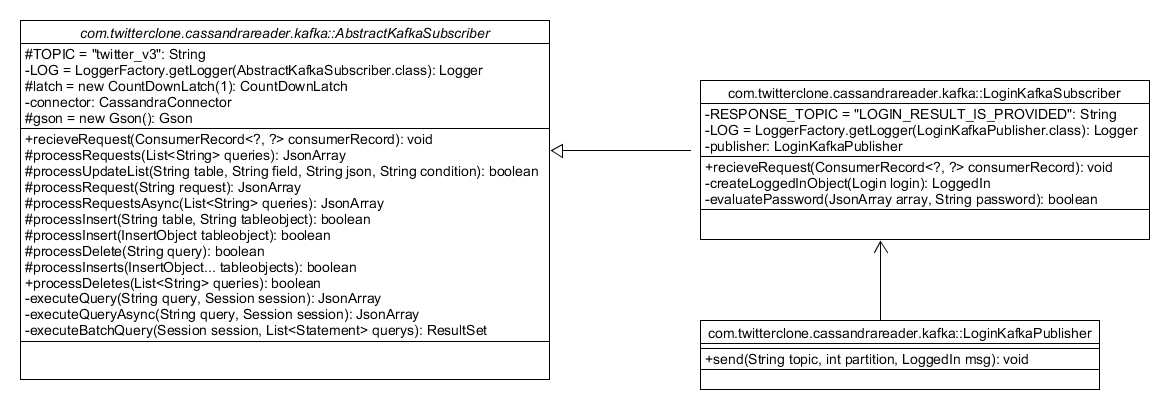
\includegraphics[scale=0.3]{pics/cassandrareader_architecture.png}
	\caption{Architektur der Publisher und Subscriber am Beispiel Login}
	\label{fig:archCass}
\end{figure}
Alle möglichen Anfragen und Antworten über Kafka sind als Java Klassen modelliert und können über Getter-Methoden abgefragt werden. Jeder der abgeleiteten Subscriber besitzt einen Publisher, über den die Antwort, durch Gson konvertiert, wieder versendet werden kann. Die Konfigurationsparameter sind in der Datei application.properties abgelegt und werden in den einzelnen Klassen angesprochen.


\section{Use Cases}
\label{sec:usecase}
Bei der Identifizierung der Use Cases, die für Cassandra relevant sind, haben wir uns für die Funktionen entschieden, die für einen Twitter-Client nach MVP-Prinzip (Minimal Viable Product) notwendig sind. Dabei haben wir vor allem die dazu gehören folgende Funktionen identifiziert:
\begin{itemize}
	\item Registrierung von User
	\item Anmelden von Usern
	\item Abfragen von Usern
	\item Absenden/Speichern von Tweets
	\item Abrufen der Timeline
	\item Folgen von Usern
\end{itemize}
Diese Schnittstellen machen es möglich die Grundfunktionen, also das Erstellen eines Users, das Anmelden des Users, das Senden und Lesen von Tweets über die Timeline von außen über vordefinierte Kafka Nachrichten anzusprechen.
Als weitere Schnittstellen für erweiterte Funktionen haben wir eine API für Volltextsuche über Elasticsearch gebaut, die die normale Volltextsuche aber auch Autocompletion unterstützt.\\

\subsection{Registrierung von Usern}
Die Registrierung von Usern bringt einen direkten Zugriff auf die Datenbank mit sich. Zunächst muss der User seine Anmeldedaten in unserem Frontend hinterlegen. Schickt er diese, bekommt der Cassandrareader über eine Zwischenstelle eine Nachricht über Kafka auf dem Topic "USER\_ISSUES\_ REGISTRATION". Diese Nachricht enthält alle relevanten Daten wie Name, Username, Hashwert des Passworts, etc. die das System braucht um den User anzulegen. Der Cassandrareader reagiert auf diese Nachricht, indem er den User in den in Abschnitt \ref{subsec:schema} genannten Tabellen für die User ablegt. Der Cassandrareader schickt eine Nachricht auf dem Topic "REGISTRATION\_RESULT\_PROVIDED" als Bestätigung zurück, ob der User erfolgreich in beide Tabellen eingetragen wurde oder nicht. Basierend auf dieser Nachricht wird im Frontend angezeigt, ob die Registrierung erfolgreich war.

\subsection{Anmelden von Usern}
Die Anmeldung von Usern geschieht über den einzigartigen Username und ein selber gewähltes Passwort. Diese Informationen werden vom Frontend weitergeleitet und kommen beim Cassandrareader in einer Kafka Nachricht auf dem Topic "USER\_ISSUES\_LOGIN" an. Diese Nachricht enthält nur den Username und das gehashte Passwort. Das gehashte Passwort wird mit dem verglichen, das in der Tabelle user\_by\_screen\_name gespeichert ist. Auch hier findet sich nur ein Hashwert des Passworts. Sind die Werte gleich, so gibt es hier eine Übereinstimmung und der Login kann genehmigt werden. Als Bestätigung dieses Vorgangs schickt der Cassandrareader eine Nachricht zurück, in der es eine Boolean Feld für das Login Ergebnis gibt. War der Login erfolgreich wird das Feld true, sonst false. Diese Nachricht wird vom Cassandrareader wieder über das Topic "LOGIN\_RESULT\_IS\_PROVIDED" verbreitet und somit auch an das Frontend weitergeleitet, das das Ergebnis darstellt und darauf reagiert.

\subsection{Abfragen von Usern}
\label{subsec:Userabfrage}
Das Abfragen von Usern braucht man vor allem, wenn man die Seite eines Users mit allen seinen Informationen aufrufen möchte. Dazu verarbeitet der Cassandrareader Nachrichten auf dem Topic "USER\_OPENS\_USER\_PAGE" in der eine User-Id angegeben ist, so dass er eine Abfrage auf Cassandra startet, in der er den User aus user\_by\_id abfragt. Dieser User wird dann als JSON in einer Kafka Nachricht über das Topic "USER\_PAGE\_ENTRIES\_ PROVIDED" wieder verbreitet. So können die Information dann vom Frontend dann z.B. als User Seite verarbeitet werden.\\
Ein ähnlicher Use Case ist die Suche nach Usern. Der Cassandrareader bekommt auf dem Topic "USER\_SEARCH\_ISSUED" eine Nachricht mit einem Usernamen. Da die Tabelle user\_by\_screen\_name nach Usernamen filterbar ist, kann der Cassandrareader eine effiziente Abfrage auf der Tabelle ausführen, die alle mit dem Namen aus der Nachricht übereinstimmenden User zurückgibt und danach den besten möglichen auswählt. Dieser wird dann in einer Nachricht auf dem Topic "USER\_SEARCH\_RESULT\_ PROVIDED" zurückgeschickt und kann dann weiterverarbeitet werden.

\subsection{Absenden/Speichern von Tweets}
\label{subsec:Tweetabfrage}
Das Absenden von Tweets ist im Endeffekt nichts anderes als ein Einfügen eines Tweets in die Datenbank. Da wir hier aber nicht mit einer relationalen Datenbank arbeiten, muss man Einfügen vor allem auf die Konsistenz des Datenschemas achten. Jeder Tweet muss nach dem Schema unabhängig voneinander in jedem der drei Tweet Tabellen richtig abgelegt werden. Dafür bekommt der Cassandrareader das Tweet Objekt über Kafka auf dem Topic "USER\_ISSUES\_TWEET" zugeschickt. Dieses Objekt wird dann mit dem Absender als User in die Tabelle tweets\_by\_tweeted eingefügt. Zusätzlich lesen wir alle Hashtags des Tweets aus und speichern ihn in der Tabelle tweets\_by\_hashtag noch einmal für jeden Hashtag, das beschleunigt das Auslesen nach Hashtags. Als letztes wird der Tweet auch noch einmal in der Tabelle tweets\_by\_follower abgespeichert, in der jeder Tweet eines Users für jeden User, der ihm folgt, abgespeichert werden. Dafür müssen natürlich zunächst erst einmal alle Follower des Absenders abgefragt werden, bevor der Tweet für sie gespeichert werden kann. Diese redundante Speicherung von Tweets beschleunigt das Auslesen für spezifische und oft gebrauchte Use Cases ungemein und hat für uns die damit einhergehenden Performance Nachteile beim Speichern von Tweets überwogen. Der Cassandrareader führt diese Einfüge Operationen durch und bestätigt über Kafka auf dem Topic "TWEET\_SAVED", ob das Speichern erfolgreich war oder nicht.


\subsection{Abrufen der Timeline}
\label{subsec:Timeline}
Das Abrufen der Timeline ist einer der zentralen Use Cases unserer Anwendung, da sie der erste Teil ist, den User innerhalb unserer Anwendung sehen und die Basis für jede Aktion nach dem Anmelden ist. Die Timeline eines Users besteht aus den Tweets aller User, denen der eingeloggte User folgt. Daher müsste man diese User zunächst aus der Datenbank abfragen und dann für jeden einzelnen eine einzelne Abfrage starten. Um uns diesen Umweg zu sparen, pflegen wir die Tabelle tweets\_by\_follower. Somit können wir, um die Timeline aufzurufen, einfach eine Abfrage auf diese Tabelle ausführen und bekommen somit direkt den Inhalt der Timeline. Wir nehmen dabei für das Speichern von Tweets mehr Datenbankzugriffe und Redundanzen in Kauf, wie in Unterabschnitt \ref{subsec:Tweetabfrage} beschrieben, um das Auslesen so effizient wie möglich zu gestalten. Die so abgefragten Tweets werden danach als JSON verpackt und auf dem Topic "TIMELINE\_ENTRIES\_PROVIDED" verbreitet. So kann die Nachricht zum Frontend propagiert werden, das dann die Timeline anzeigt.


\subsection{Folgen von Usern}
Das Folgen von Usern bestimmt vor allem den Aufbau der Timeline, da hier, wie in Unterabschnitt \ref{subsec:Timeline} erwähnt, alle Tweets der gefolgten User angezeigt werden. Um das Folgen von Usern umsetzen zu können, erhält der Cassandrareader einer Nachricht auf dem Topic "USER\_WANTS\_TO\_FOLLOW\_ USER", in der die User-Id des anderen Users und des eigenen steht. Followers werden in unserem Datenschema für jeden User als Liste gespeichert, einmal alle User, denen ein User folgt, und alle User, die einem User folgen. Jeder Eintrag für einen User in den Tabellen user\_by\_id und user\_by\_screen\_name enthält beide Listen. Außerdem enthält das User Profil einen Follower Count und eine Friends Count, der die Anzahl User zählt denen man selber folgt. Der Cassandrareader führt auf beiden Tabellen für jede Folgen Anfrage folgende Aktion durch. Er erhöht beim eigenen User den Friends Count und beim User, dem gefolgt werden soll, den Follower Count. Danach wird das User Profil des Users, dem gefolgt werden soll, in die Friends Liste des anfragenden Users hinzugefügt und das Profil des anfragenden Users in die Follower Liste der zu folgenden Users. Geschieht das alles ohne Fehler bestätigt der Cassandrareader die Anfrage auf dem "USER\_FOLLOWS\_USER" Topic positiv.
